\subsection{Phương pháp mã hóa và giải mã mạng neural nhiều lớp trong không gian chung}
\subsubsection{Mã hóa cá thể}
Khi ANN chỉ có 1 lớp, điểm khác nhau duy nhất giữa các cấu hình mạng giữa các tác vụ là ở số đơn vị xử lý trong lớp ẩn. Cách mã hóa của Chandra et al\cite{chandra2018evolutionary} xuất phát từ một mạng cơ bản nhỏ nhất trong không gian chung, sau đó cứ mỗi đơn vị xử lý thêm vào, họ bổ sung thêm các tham số tương ứng với các kết nối từ nó đến các lớp đầu vào và lớp đầu ra vào phần cuối của kiểu gen. Cách làm này sẽ không còn phù hợp khi khi số lớp tăng lên và đặc biệt là khi cấu hình ANN của các tác vụ khác nhau về số lớp. 
\begin{figure}[h!]
    \centering
    \fbox{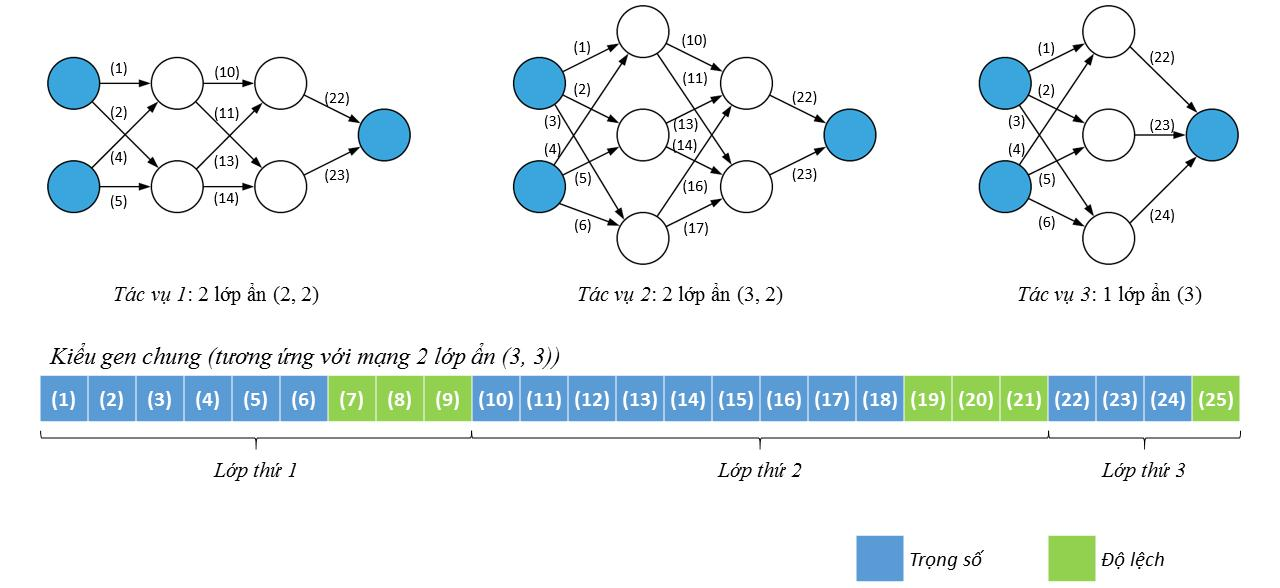
\includegraphics[width=1.0\linewidth]{thesis/images/encode.jpg}}
    \caption{Phương pháp mã hóa các ANN khác cấu trúc trong cùng không gian chung.}
    \label{fig:encode}
\end{figure}
Bởi vậy trong nghiên cứu gần đây về huấn luyện ANN nhiều lớp Tuan NQ and Thanh Le\cite{nqtuan} đã đưa ra một phương pháp mã hóa mới. Hình \ref{fig:encode} minh họa cách mã hóa này cho 3 mạng thuộc 3 tác vụ tối ưu đa nhiệm khác nhau có cấu hình rút gọn là: $H_1 = (2,2), H_2=(3,2), H_3=(3)$. Cách mã hóa này sẽ dựa vào việc xác định cấu hình chung cho các ANN và từ cấu hình chung này xây dựng cá thể.
\subsubsection{Xây dựng không gian chung}
Một kiểu gen chung được đưa ra cho tất cả các mạng thành phần và cách chiều các thành phần trọng số cũng như độ lệch của mạng lên kiểu gen chung được thể hiện bằng các con số tương ứng.
Trực quan ta thấy kiểu gen chung ở đây là cấu hình ANN có số lớp lớn nhất và số các đơn vị xử lý thành phần cũng lớn nhất. Giải thuật \ref{h-multi} \cite{nqtuan} thực hiện chính xác cách xác định cấu hình chung ANN chung lớn nhất.
\begin{algorithm} [h!]
    \caption{Tính $H_{multitask}$, bao gồm các tham số của không gian biểu diễn chung}
    \textbf{Đầu vào}: $H_j$ với $j \in [1, K]$\\
    \textbf{Đầu ra}: $H_{multitask}$
    \begin{algorithmic}[1]
        \State $h_{multitask}^{(0)} = $ Số chiều của lớp đầu vào;
        \State $h_{multitask}^{(\theta)} = \max_{j \in [1, K]} h_j^{(l_j)}$;
        \For{$i = 1 \rightarrow \theta - 1$}
            \State $h_{multitask}^{(i)} = \max_{j \in [1, K]}{h_j^{(i)}}$;
        \State $h_{multitask}^{(\theta + 1)} = 1$;
        \State
    \end{algorithmic}
    \label{h-multi}
\end{algorithm}

\begin{figure}[h!]
    \centering
    \fbox{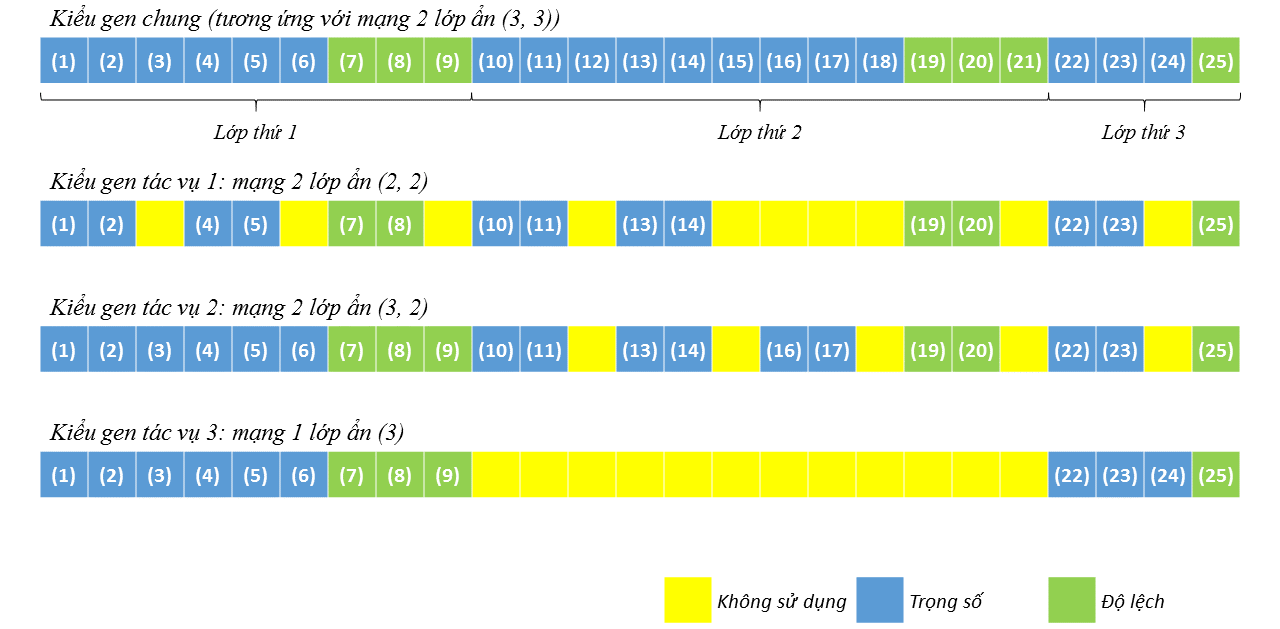
\includegraphics[width=1.0\linewidth]{thesis/images/decode.jpg}}
    \caption{Giải mã ý nghĩa của từng gen đối với mỗi tác vụ với phương pháp mã hóa.}
    \label{fig:decode}
\end{figure}

Một điểm cần lưu ý trong giải thuật \ref{h-multi} đó là với những ANN có ít lớp hơn, ta chia chia sẻ tham số ở lớp cuối của chúng với cấu hình mạng chung lớn nhất chứ không phải theo chỉ số của lớp đó. Cách làm này có ý nghĩa rất quan trọng vì việc chia sẻ trọng số lớp nào đi với lớp đó: lớp đầu vào đi với lớp đầu vào, lớp đầu ra đi với lớp đầu ra, các lớp ẩn thì lần lượt từ trước đến sau. 
\subsubsection{Giải mã cá thể}
Sau khi có được mã hóa chung của tất cả các ANN, mỗi ANN của các tác vụ khác nhau có vị trí các trọng số được sử dụng trong kiểu gen chung khác nhau như trong \ref{fig:decode}. Khi cần giải mã cá thể trở về cấu hình mạng tương ứng của từng tác vụ ta dựa vào cấu hình ANN của tác vụ đó và cấu hình ANN biểu diễn chung giữa các tác vụ.

Để tăng hiệu quả của phép biểu diễn chung khi áp dụng các toán tử di truyền, giá trị của mỗi biến trên gen được giới hạn đồng nhất trong khoảng $[0,1]$. Kiểu hình tương ứng sẽ được biến đổi mở rộng ra một khoảng giá trị $[y_1, y_2]$ với $y_1, y_2 \in \mathbb{R}$ bằng một phép biến đổi đơn giản $X = (y_2-y_1) x + y_1$. Cách làm này cũng được sử dụng trong phần lớn các giái thuật tiến hóa đa nhiệm cho không gian số thực.


% \begin{example}
%     Giả sử ta có 3 task có cấu trúc mạng tương ứng với $H_1 = [2, 2, 2, 1]$, $H_2 = [2, 3, 2, 1]$ và $H_3 = [2, 3, 1]$.
%     Theo thuật toán (\ref{h-multi}) thì ta có $H_{multitask}=[2, 3, 3, 1]$. Từ $H_{multitask}$ ta có thể tính được tổng số tham số trong mạng nơ-ron là (tính cả weights và bias): $2 \cdot 3 + 3 + 3 \cdot 3 + 3 + 3 \cdot 1 + 1 = 25$

%     Một kiểu gen sẽ có thể được biểu diễn như dưới đây (lần lượt theo thứ tự của các weights và bias):
%     \begin{equation}
%       genotype=
%       \begin{bmatrix}
%         1& 2& 3& \dots & 25
%       \end{bmatrix}
%     \end{equation}
    
%     \label{ex1}
%   \end{example}
%   \begin{figure}[h!] 
%     \centering
%     \fbox{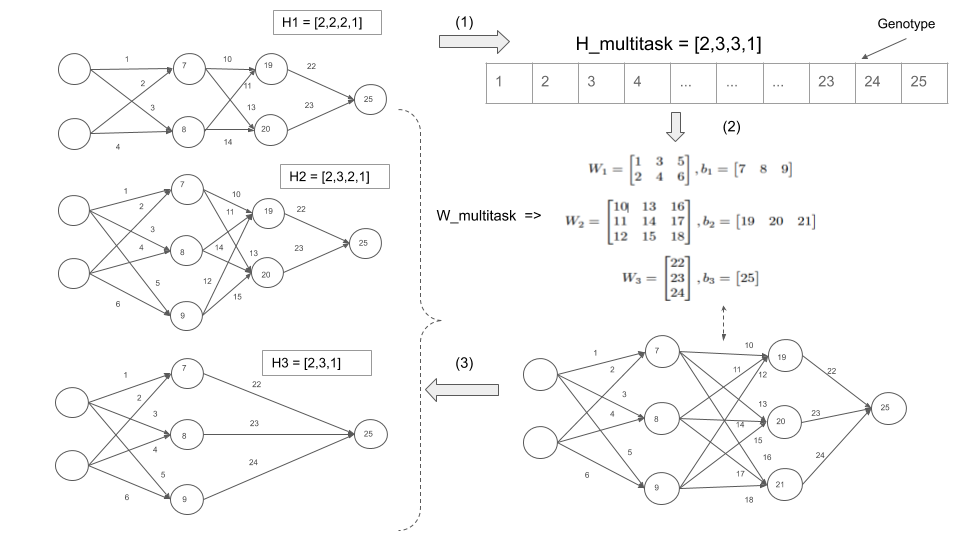
\includegraphics[width=1.0\linewidth]{modular-ex.png}}
%     \caption{Ví dụ thuật toán giải mã đề xuất cho các mô hình mạng H1(2,2,2,1), H2(2,3,2,1), H3(2,3,1)}
%     \label{fig:problem:modular-ex1}
% \end{figure}
 
%   \begin{algorithm}[h!] 
%   \caption{Generate $W_{multitask}$, which is list of weight matrices according to $H_{multitask}$}
%   \textbf{Input}: $genotype$ and $H_{multitask}$\\
%   \textbf{Output}: $W_{multitask}$
%   \begin{algorithmic}[1]
%     \State $base = 0$
%     \For{$i = 1 \rightarrow \theta + 1$}
%       \State $in = h_{multitask}^{(i-1)}$
%       \State $out = h_{multitask}^{(i)}$
%       \State $W_{multitask}^{(i)} = genotype[base: base + in * out]$
%       \State $W_{multitask}^{(i)} = W_{multitask}^{(i)}.reshape(in, out)$
%       \State $base = base + in * out$
%       \State $b_{multitask}^{(i)} = genotype[base: base + out]$
%       \State $base = base + out$
%     \EndFor
%   \end{algorithmic}
%   \label{alg3}
%   \end{algorithm}

%   \begin{example}
%     Tiếp theo ví dụ \ref{ex1} dựa theo thuật toán \ref{alg3}, ta tính được trọng số \emph{multitask} như sau:
%     \begin{equation}
%       W_1=
%       \begin{bmatrix}
%         1& 3& 5\\
%         2& 4& 6
%       \end{bmatrix},
%       b_1=
%       \begin{bmatrix}
%         7& 8& 9
%       \end{bmatrix}
%     \end{equation}

%     \begin{equation}
%       W_2=
%       \begin{bmatrix}
%         10& 13& 16\\
%         11& 14& 17\\
%         12& 15& 18
%       \end{bmatrix},
%       b_2=
%       \begin{bmatrix}
%         19& 20& 21\\
%       \end{bmatrix}
%     \end{equation}

%     \begin{equation}
%       W_3=
%       \begin{bmatrix}
%         22\\
%         23\\
%         24
%       \end{bmatrix},
%       b_3=
%       \begin{bmatrix}
%         25
%       \end{bmatrix}
%     \end{equation}
%     \label{ex2}
%   \end{example}

%   \begin{algorithm}[h!] 
%   \caption{Select and slice the $W_{multitask}$ to obtain $W_{j}$, which is list of weight matrices according to $H_{j}$}
%   \textbf{Input}: $W_{multitask}$ and $H_j$\\
%   \textbf{Output}: $W_j$
%   \begin{algorithmic}[1]
%     \For{$i = 1 \rightarrow l_j$}
%       \State $in = h_j^{(i-1)}$
%       \State $out = h_j^{(i)}$
%       \State $W_j^{(i)} = W_{multitask}^{(i)}[:in, :out]$ \Comment{Parameters are shared between corresponding layers}
%       \State $b_j^{(i)} = b_{multitask}^{(i)}[:out]$
%     \EndFor
%     \State $W_j^{(l_j + 1)} = W_{multitask}^{(\theta+1)}[:in, :out]$ \Comment{Except for tasks have different number of layers, parameters are also shared between their last layers}
%     \State $b_j^{(l_j + 1)} = b_{multitask}^{(\theta+1)}[:out]$
%   \end{algorithmic}
%   \label{alg4}
%   \end{algorithm}

%   \begin{example}
%     Tiếp tục ví dụ \ref{ex2}, Dựa theo thuật toán \ref{alg4}, bộ trọng số \emph{w,b} của mỗi tác vụ sẽ được giải mã như sau:

%     \textbf{Task1}: $H_1 = [2, 2, 2, 1]$
%     \begin{equation}
%       W_1=
%       \begin{bmatrix}
%         1& 3\\
%         2& 4
%       \end{bmatrix},
%       b_1=
%       \begin{bmatrix}
%         7& 8
%       \end{bmatrix}
%     \end{equation}

%     \begin{equation}
%       W_2=
%       \begin{bmatrix}
%         10& 13\\
%         11& 14\\
%         12& 15
%       \end{bmatrix},
%       b_2=
%       \begin{bmatrix}
%         19& 20\\
%       \end{bmatrix}
%     \end{equation}


%     \begin{equation}
%       W_3=
%       \begin{bmatrix}
%         22\\
%         23
%       \end{bmatrix},
%       b_3=
%       \begin{bmatrix}
%         25
%       \end{bmatrix}
%     \end{equation}


%     \textbf{Task2}: $H_2 = [2, 3, 2, 1]$
%     \begin{equation}
%       W_1=
%       \begin{bmatrix}
%         1& 3& 5\\
%         2& 4& 6
%       \end{bmatrix},
%       b_1=
%       \begin{bmatrix}
%         7& 8& 9
%       \end{bmatrix}
%     \end{equation}

%     \begin{equation}
%       W_2=
%       \begin{bmatrix}
%         10& 13\\
%         11& 14\\
%         12& 15
%       \end{bmatrix},
%       b_2=
%       \begin{bmatrix}
%         19& 20\\
%       \end{bmatrix}
%     \end{equation}


%     \begin{equation}
%       W_3=
%       \begin{bmatrix}
%         22\\
%         23
%       \end{bmatrix},
%       b_3=
%       \begin{bmatrix}
%         25
%       \end{bmatrix}
%     \end{equation}

%     \textbf{Task3}: $H_3 = [2, 3, 1]$
%     \begin{equation}
%       W_1=
%       \begin{bmatrix}
%         1& 3& 5\\
%         2& 4& 6
%       \end{bmatrix},
%       b_1=
%       \begin{bmatrix}
%         7& 8& 9
%       \end{bmatrix}
%     \end{equation}

%     \begin{equation}
%       W_2=
%       \begin{bmatrix}
%         22\\
%         23\\
%         24
%       \end{bmatrix},
%       b_2=
%       \begin{bmatrix}
%         25
%       \end{bmatrix}
%     \end{equation}

%   \end{example}
\subsection{Tính toán độ thích nghi}
\label{fitness}
Các cá thể $x$ trong quần thể $P$ đều được gắn với một tác vụ tối ưu hóa tương ứng với chỉ số kỹ năng của chúng. Từ chỉ số kĩ năng này của 1 cá thể $x$, ta xác định được cấu hình ANN đầy đủ $H_x$ của $x$. Thêm vào đó, với mỗi cá thể $x$, ta xác định được kiểu hình $\mathcal{X}$ tương ứng chứa tất cả các tham số quyết định của mô hình mạng là $W$ và độ lệch $b$.
Từ $W$ và $b$ thu được, ta áp dụng để tính giá trị hàm mất mát như đã trình bày ở trên. Trong khuôn khổ của đồ án, tôi chỉ tập trung thực nghiệm trên các bài toán phân loại nhị phân, do đó hàm mất mát được sử dụng chính là $MSE$ đã trình bày ở công thức . Giá trị hàm mất mát này chính là độ thích nghi đơn nhiệm của cá thể $x$. 

\subsection{Chiến lược tiến hóa đa nhiệm đề xuất}
Về cơ bản giải thuật tiến hóa đa nhiệm đề xuất để huấn luyện nhiều ANN khác cấu trúc đồng thời sẽ dựa theo khung thuật toán MFEA-II đã trình bày ở mục \ref{section:mfeaii}. Và cơ chế chọn lọc cá thể tối ưu trên không gian đa nhiệm theo đánh giá độ thích nghi vô hướng với những điều chỉnh phù hợp cho bài toán huấn luyện ANN. 
Các bước giải quyết bài toán được biểu diễn theo thứ tự như trong giải thuật \ref{alg:proposed-alg1}.
\begin{algorithm} [h!]
    \caption{Các bước chính của giải thuật tiến hóa đa nhiệm huấn luyện nhiều ANN khác cấu trúc}
    \begin{algorithmic}[1]
        \State Xác định không gian biểu diễn chung theo giải thuật \ref{h-multi}
        \State Khởi tạo các cá thể ngẫu nhiên của từng tác vụ theo phân phối chuẩn \ref{h-multi}
        \State Gán chỉ số kỹ năng cho mỗi cá thể
        \State Đánh giá giá trị thích nghi đơn nhiệm mỗi cá thể theo chỉ số kỹ năng tương ứng
        \For{Điều kiện dừng}
            \State Xáo trộn thứ tự ngẫu nhiên các cá thể trong quần thể $P$
            \State Xác định tập các cá thể thuộc từng tác vụ
            \State Học ma trận xác suất ghép cặp $RMP$ giữa các cặp tác vụ với tập các cá thể hiện tại
            \For{Duyệt hết các cá thể trong quần thể}
                \State Chọn ngẫu nhiên $p_1, p_2$ trong quần thể $P$
                \State Lai ghép, đột biến bằng cách tổ hợp $p_1, p_2$
                \State Đánh giá giá trị thích nghi đơn nhiệm cho mỗi cá thể mới
                \State Đánh giá độ thích nghi vô hướng
                \State Chọn lọc cá thể
            \EndFor
        \EndFor
    \end{algorithmic}
    \label{alg:proposed-alg1}
\end{algorithm}

\subsubsection{Phép lai ghép, đột biến trong không gian chung}
Trong [53], Chandra et al. và N.Q.Tuan sử dụng phép lai ghép SBX và phép đột biến PMU để làm phép tìm kiếm cơ sở và không sử dụng bất cứ phép biến đổi nào dựa trên đạo hàm. Cũng theo lẽ đó, tiến hóa đa nhiệm đề xuất trong đồ án cũng không sử dụng bất cứ phép biến đổi nào dựa trên đạo hàm. Cụ thể các phép lai ghép, đột biến được sử dụng là SBX và PMU. Và để đảm bảo nguyên tắc các cá thể con cái sinh ra là parent-centric, chỉ số phân phối SBX và tỉ lệ đột biến PMU đều cần có giá trị đủ lớn. 

\subsubsection{Học ma trận $RMP$ trên số chiều của không gian chung}
Như đã trình bày, để giảm thiểu khả năng xảy ra negative transfer giữa các tác vụ trong quá trình lai ghép khác tác vụ, ta cần tính ma trận xác suất ghép cặp $RMP$ sao cho phù hợp với mối quan hệ giữa các chúng. Ta có thể tính toán cập nhật ma trận $RMP$ tại từng thế hệ bằng cách tối ưu hóa được đưa ra ở \ref{equa:true_distribution} và \ref{equa:likelihood}. Với bài toán huấn luyện nhiều ANN khác cấu trúc này đồ án sẽ xây dựng phương pháp ước lượng ma trận xác suất ghép cặp $RMP$ trên tập các cá thể của mỗi tác vụ tương ứng với từng thế hệ như trong giải thuật \ref{alg:rmp}.

\begin{algorithm}[h!]
    \caption{Tính toán ma trận RMP (Random Mating Probability)}
    \textbf{Đầu vào}: K tập hợp cá thể của từng tác vụ.\\
    D là số chiều của không gian tìm kiếm chung.\\
    \textbf{Đầu ra}: Ma trận xác suất ghép cặp ngẫu nhiên $RMP$ tương ứng với độ tương đồng giữa từng cặp tác vụ. 
    \begin{algorithmic}[1]
        \State Tính phân phối của tập các cá thể của từng tác vụ. Phân phối của tác vụ thứ $k$ có trung vị là $\m_k$ và hiệp phương sai là $\sum_k$
        \For{$k = 0 \rightarrow K-1$}
            \For{$j = k+1 \rightarrow K$}
                \State Tính xác suất tập cá thể của các tác vụ $j$ theo phân phối của tác vụ $k$ với số chiều $D$ của không gian tìm kiếm chung.
                \State Tính xác suất tập cá thể của các tác vụ $k$ theo phân phối của tác vụ $j$ với số chiều $D$ của không gian tìm kiếm chung.
                \State Tính toán xác suất ghép cặp ngẫu nhiên $rmp_{k,j}$ bằng cách tối ưu hàm $likelihood$ được mô tả trong công thức \ref{equa:true_distribution} và \ref{equa:likelihood} tương ứng với cặp tác vụ $k,j$
                \State Cập nhật vào ma trận RMP
            \EndFor
        \EndFor
    \end{algorithmic}
    \label{alg:rmp}
\end{algorithm}


